\chapter{Modellierung und Entwurf}
\label{cha:mue}

In diesem Kapitel werden die funktionalen Anforderungen aus dem Abschnitt \ref{sec:anforderungsdefinition} spezifiziert. Modelle für die einzelnen funktionalen Anforderungen sollen entwickelt werden. Die Modelle veranschaulichen das geforderte funktionale Verhalten der Software. Voraussetzung für die Entwicklung der Modelle ist die Konkretisierung der funktionalen Anforderungen. Diese Konkretisierung beinhaltet die Festlegung der Bestandteile die für eine Implementierung der funktionalen Anforderung benötigt werden. Ziel des Kapitels ist es, die wichtigsten Bestandteile einer funktionalen Anwendung herauszubilden, dieses Bestandteile zu definieren und zu veranschaulichen.

\section{Computerspiele}
\label{sec:computerspiele}

In diesem Abschnitt werden die Bestandteile der Computerspiele festgelegt und veranschaulicht. 

\subsection{Tic Tac Toe}
\label{sec:ttt}

Das klassische Tic Tac Toe ist ein Spiel, welches mit genau zwei Spielern gespielt wird. Jeder dieser Spieler zeichnet abwechselnd entweder ein Kreuz oder einen Kreis in eine Matrix auf ein Blatt Papier. Während eines gesamten Spiels darf ein Spieler nur Kreuze zeichnen und der andere Spieler nur Kreise. Das Spielfeld ist eine drei mal drei große Matrix, also können maximal neun Symbole in diese Matrix eingetragen werden. Um die Anzahl der möglichen Spielzüge zu erhöhen wird das Spielfeld des klassischen Tic Tac Toe auf eine vier mal vier Matrix erweitert.

\myparagraph{Spielregeln}

Ziel des Spiels ist es vier Kreuze oder vier Kreise in einer bestimmten Position anzuordnen. Im nachfolgenden wird davon ausgegangen, dass der menschliche Spieler Kreuze verwendet und der Computergegner Kreise. Die Kreise und Kreuze sind Spielfiguren, welche den jeweiligen Spieler repräsentieren. Der menschliche Spieler hat zusätzlich, in den Nachfolgenden Siegesszenarien, das Anrecht auf den ersten Zug. Es existieren drei unterschiedliche Anordnungen von Spielfiguren, die das Spiel beenden und einen Sieg herbeiführen. Gewinnt ein Spieler mit einer Siegesanordnung seiner Spielfiguren, dann verliert der andere Spieler dadurch automatisch.

Eine horizontale Siegesanordnung entsteht, wenn vier Spielfiguren eines Spielers in einer horizontalen Reihe, veranschaulicht in Abbildung \ref{fig:tttHorizontalerSieg}, angeordnet sind. In jeder Reihe des Spielbretts ist ein horizontaler Sieg möglich.

\begin{figure}[!htbp]
  \centering
  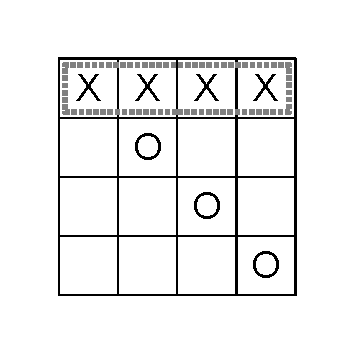
\includegraphics[scale = 1]{inhalt/abbildungen/horizontaler_sieg.pdf}
  \caption{Tic Tac Toe horizontaler Sieg}
  \label{fig:tttHorizontalerSieg}
\end{figure}

In Abbildung \ref{fig:tttVertikalerSieg} gewinnt der menschliche Spieler knapp gegen den Computergegner mit einer ununterbrochenen vertikalen Reihe. Der Computergegner hätte fast eine diagonale Reihe aus Kreisen verbunden, die jedoch von dem menschlichen Spieler mit einer Spielfigur geblockt wurde. Zudem hätte der Computergegner auch fast eine vertikale Reihe ohne Unterbrechungen vervollständigt.

\begin{figure}[!htbp]
  \centering
  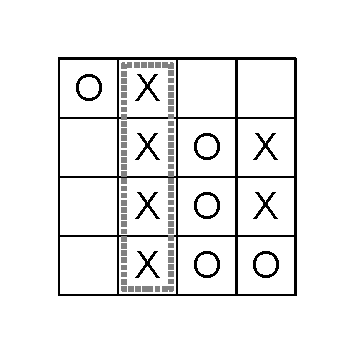
\includegraphics[scale = 1]{inhalt/abbildungen/vertikaler_sieg.pdf}
  \caption{Tic Tac Toe vertikaler Sieg}
  \label{fig:tttVertikalerSieg}
\end{figure}

Die dritte und letzte Anordnungsvariante der Spielfiguren, welche zu einem Sieg eines Spielers führt, ist die diagonale Verbindung von vier Spielfiguren eines Spielers. In Abbildung \ref{fig:tttDiagonalerSieg} gewinnt der Computergegner mit einer diagonalen Anordnung von vier Spielfiguren ohne Unterbrechung einer gegnerischen Spielfigur.

\begin{figure}[!htbp]
  \centering
  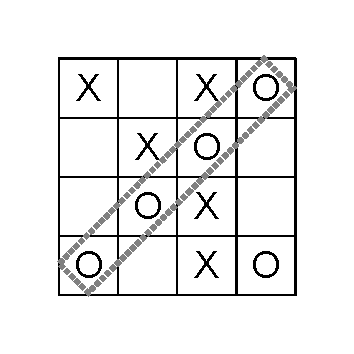
\includegraphics[scale = 1]{inhalt/abbildungen/diagonaler_sieg.pdf}
  \caption{Tic Tac Toe diagonaler Sieg}
  \label{fig:tttDiagonalerSieg}
\end{figure}

Insgesamt existieren vier vertikale, vier horizontale und zwei diagonale Anordnungen der Spielfiguren, welche einen Sieg herbeiführen würden, also zehn verschiedene Siegesanordnungen. Was passiert jedoch, wenn keine der zehn möglichen Siegesanordnungen auftritt?

Dann gewinnt bzw. verliert keiner der beiden Spieler und es entsteht ein Unentschieden. Sind die beiden Kontrahenten gleich gut, erfahren oder verwenden die selben Strategien, dann tritt ein Unentschieden möglicherweise öfter oder andauernd ein.

\myparagraph{Benutzerschnittstellen}

Der Benutzer kann seine Kreuze auf das Spielbrett setzen indem er ein vorher vom Spiel definiertes Zahlentupel über die Tastatur eingibt. Welche Zahlentupel ein Kreuz an welche Stelle setzt ist in Abbildung \ref{fig:kreiseUndKreuzeSetzen} definiert. Sollte der menschliche Spieler keines der erlaubten Zahlentupel eingeben, dann wird er darauf hingewiesen, welche Steuerungsmöglichkeiten zum setzen der Spielfiguren ihm zur Verfügung stehen.

\begin{figure}[!htbp]
  \centering
  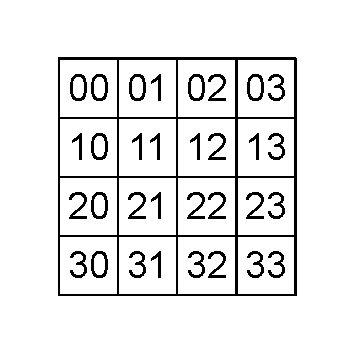
\includegraphics[scale = 1]{inhalt/abbildungen/vier_mal_vier_matrix.pdf}
  \caption{Tic Tac Toe Spielfiguren setzen}
  \label{fig:kreiseUndKreuzeSetzen}
\end{figure}

\subsection{Reversi}
\myparagraph{Spielprinzipien}
\myparagraph{Spielregeln}
\myparagraph{Benutzerschnittstellen}

\section{Lernverfahren}
\label{sec:lernverfahren}
\subsection{Analyse und Auswahl der lernfähigen Algorithmen}

\subsection{Anwendung der Algorithmen auf Computerspiele}

\subsection{Konzeptuelles Training der Algorithmen}

\subsection{Persistenz der Trainingsdaten}